\documentclass[conference]{IEEEtran}
\usepackage{amsmath,amsfonts,amssymb}
\usepackage{graphicx}
\usepackage{booktabs}
\usepackage{multirow}
\usepackage{array}
\usepackage{color}
\usepackage{url}
\usepackage{cite}
\usepackage{caption}
\usepackage{float}
\usepackage{microtype}

\hyphenation{op-tical net-works semi-conduc-tor}

\begin{document}

\title{Analyse Comparative des Algorithmes de Classification Supervisée pour le Diagnostic du Cancer du Sein}

\author{\IEEEauthorblockN{Sohayeb Gasmi}
\IEEEauthorblockA{Département d'Informatique\\
Université\\
Email: sohayeb.gasmi79@gmail.com}
}

\maketitle

\begin{abstract}
Ce travail présente une étude comparative approfondie de six algorithmes d'apprentissage supervisé pour la classification de tumeurs mammaires (bénignes vs malignes) à partir du jeu de données Breast Cancer Wisconsin. Les modèles évalués sont : la régression logistique, KNN, l'arbre de décision, la forêt aléatoire, SVM et XGBoost. Notre méthodologie intègre des techniques avancées de prétraitement, d'optimisation des hyperparamètres, de validation croisée stratifiée, ainsi que des méthodes d'interprétabilité. Les résultats montrent que Random Forest atteint les meilleures performances avec un F1-score de 0,993. L'analyse des courbes d'apprentissage et des matrices de confusion révèle que les modèles ensemblistes présentent la meilleure robustesse et généralisation.
\end{abstract}

\section{Introduction}

Le cancer du sein représente l'un des cancers les plus fréquents chez la femme. Le diagnostic précoce et précis est crucial pour améliorer le pronostic et la survie des patients. L'analyse automatisée des caractéristiques des tumeurs par des algorithmes d'apprentissage automatique offre une opportunité majeure d'assister les professionnels de santé.

L'objectif de ce travail est triple :
\begin{enumerate}
\item Mettre en œuvre et comparer six algorithmes de classification supervisée ;
\item Analyser l'impact des étapes de prétraitement, en particulier la standardisation ;
\item Proposer un cadre d'évaluation robuste intégrant des métriques avancées.
\end{enumerate}

\section{État de l'art}

\subsection{Régression Logistique}

La régression logistique est un modèle linéaire probabiliste qui estime la probabilité qu'une instance appartienne à une classe donnée \cite{hastie2009} :

\begin{equation}
P(y=1|\mathbf{x}) = \frac{1}{1 + e^{-(\beta_0 + \boldsymbol{\beta}^T \mathbf{x})}}
\end{equation}

\subsection{K-Nearest Neighbors (KNN)}

KNN classifie une instance selon la classe majoritaire de ses $k$ plus proches voisins \cite{cover1967}. La distance euclidienne est utilisée :

\begin{equation}
d(\mathbf{x}_i, \mathbf{x}_j) = \sqrt{\sum_{m=1}^{M} (x_{im} - x_{jm})^2}
\end{equation}

\subsection{Forêt Aléatoire (Random Forest)}

La forêt aléatoire, proposée par Breiman \cite{breiman2001}, agrège plusieurs arbres décorrélés. L'indice de Gini pour un nœud est :

\begin{equation}
Gini = 1 - \sum_{k=1}^{K} p_k^2
\end{equation}

\subsection{Support Vector Machine (SVM)}

SVM recherche l'hyperplan séparateur qui maximise la marge \cite{cortes1995} :

\begin{equation}
\begin{aligned}
\min_{\mathbf{w},b,\xi} \quad & \frac{1}{2}\|\mathbf{w}\|^2 + C\sum_{i=1}^{n}\xi_i \\
\text{t.q.} \quad & y_i(\mathbf{w}^T\mathbf{x}_i + b) \geq 1 - \xi_i, \; \xi_i \geq 0
\end{aligned}
\end{equation}

\subsection{XGBoost}

XGBoost est une implémentation optimisée du gradient boosting \cite{chen2016} :

\begin{equation}
\mathcal{L} = \sum_{i=1}^{n} \ell(y_i, \hat{y}_i^{(t)}) + \sum_{k=1}^{T} \Omega(f_k)
\end{equation}

\section{Méthodologie}

\subsection{Jeu de données}

Le dataset Breast Cancer Wisconsin \cite{wolberg1995} contient des caractéristiques calculées à partir d'images numérisées. Le Tableau~\ref{tab:dataset} résume ses propriétés.

\begin{table}[H]
\centering
\caption{Caractéristiques du jeu de données}
\label{tab:dataset}
\begin{tabular}{l|c}
\toprule
Propriété & Valeur \\
\midrule
Nombre d'échantillons & 569 \\
Nombre de caractéristiques & 30 \\
Classe 0 (Maligne) & 212 (37,3\%) \\
Classe 1 (Bénigne) & 357 (62,7\%) \\
Valeurs manquantes & 0 \\
\bottomrule
\end{tabular}
\end{table}

\section{Analyse exploratoire des données}

Avant d'appliquer les algorithmes de classification, une analyse exploratoire a été réalisée pour comprendre la structure et les relations entre les caractéristiques.

\subsection{Distribution des caractéristiques}

La Figure~\ref{fig:histograms} présente la distribution des caractéristiques principales du jeu de données. On observe que la plupart des caractéristiques suivent des distributions approximativement normales, avec des séparations nettes entre les deux classes pour certaines variables comme le rayon moyen et le périmètre moyen.

\begin{figure}[H]
\centering
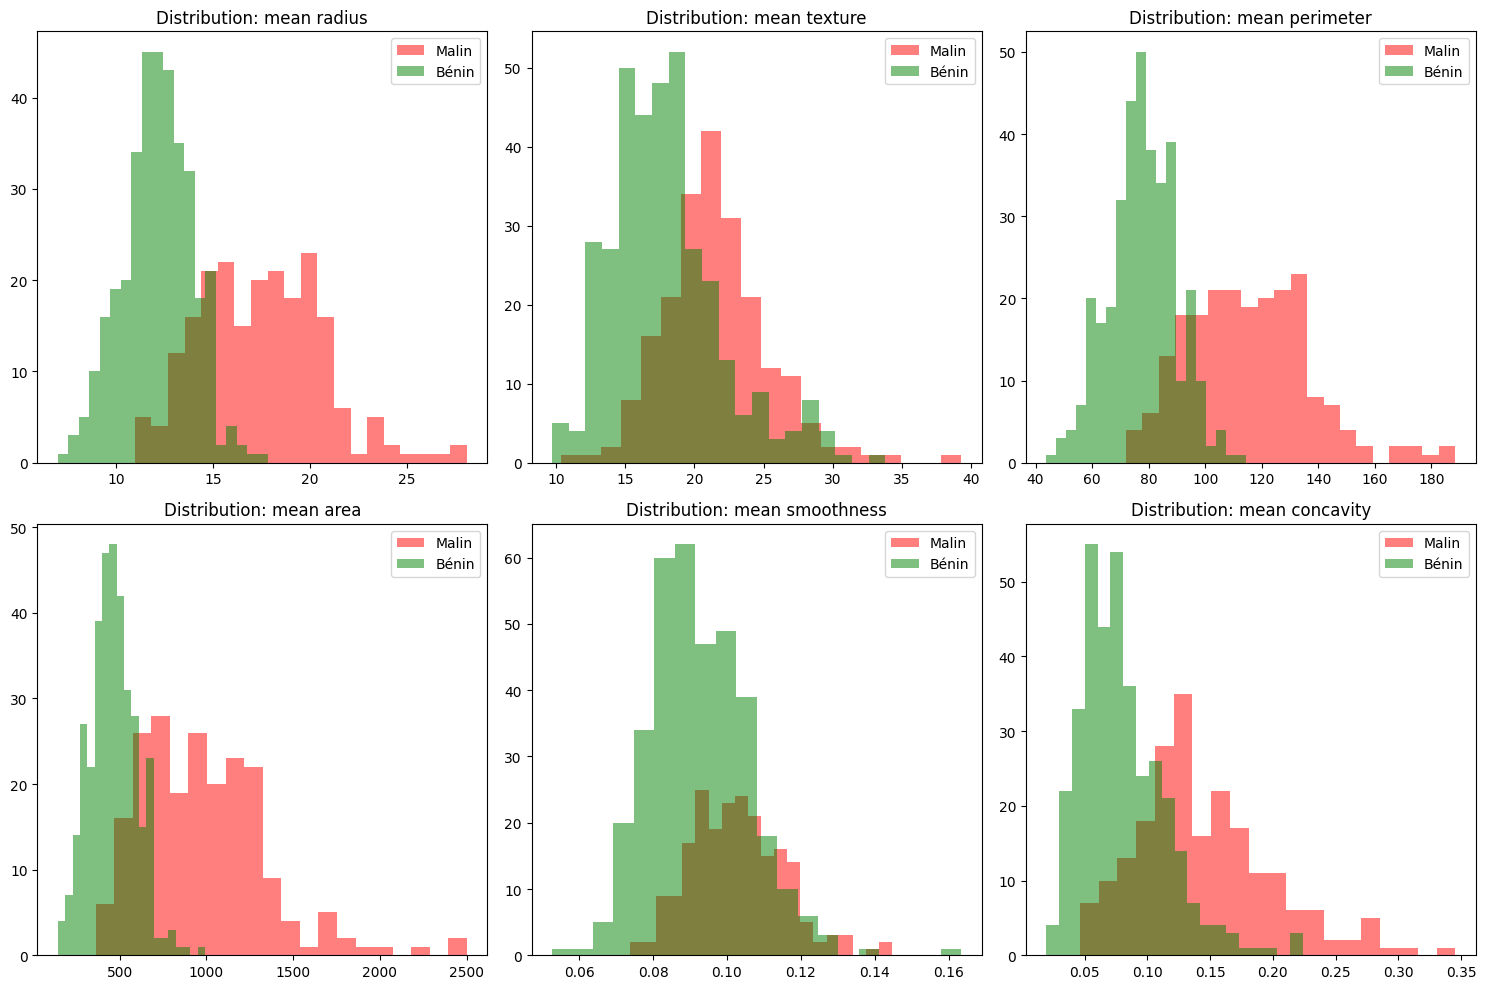
\includegraphics[width=0.95\columnwidth]{eda_histograms.png}
\caption{Distribution des caractéristiques numériques : mean radius, mean texture, mean perimeter, mean area, mean smoothness et mean concavity}
\label{fig:histograms}
\end{figure}

\subsection{Matrice de corrélation}

La Figure~\ref{fig:correlation} montre les corrélations entre les différentes caractéristiques. On note des corrélations élevées (supérieures à 0.9) entre certaines caractéristiques géométriques comme le rayon, le périmètre et la surface, suggérant une redondance potentielle qui pourrait être réduite par analyse en composantes principales.

\begin{figure}[H]
\centering
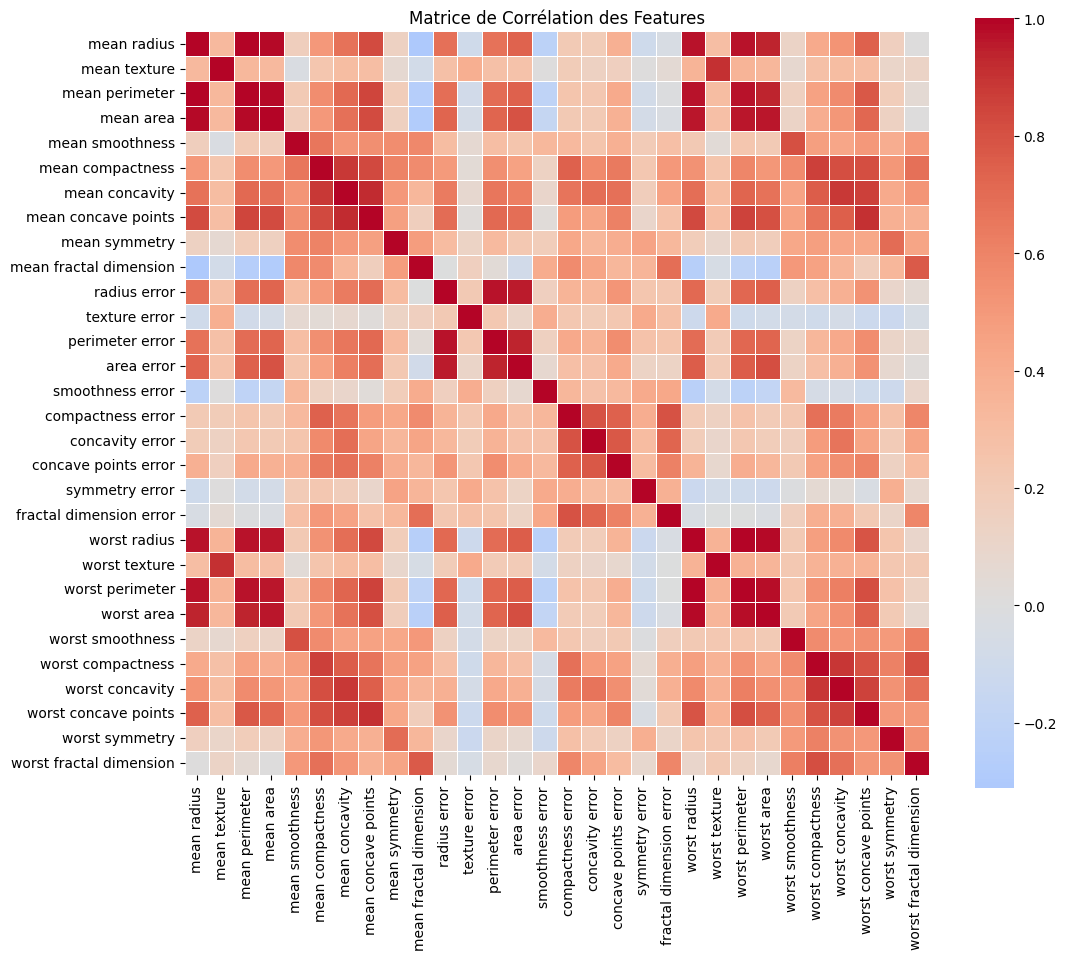
\includegraphics[width=0.95\columnwidth]{eda_correlation_matrix.png}
\caption{Matrice de corrélation des caractéristiques - Les valeurs proches de 1 (rouge) indiquent une forte corrélation positive}
\label{fig:correlation}
\end{figure}

\subsection{Analyse par boîtes à moustaches}

Les boxplots de la Figure~\ref{fig:boxplots} comparent la distribution des caractéristiques selon la classe (bénigne vs maligne). Les différences significatives entre les deux classes pour la plupart des caractéristiques indiquent leur pouvoir discriminant élevé.

\begin{figure}[H]
\centering
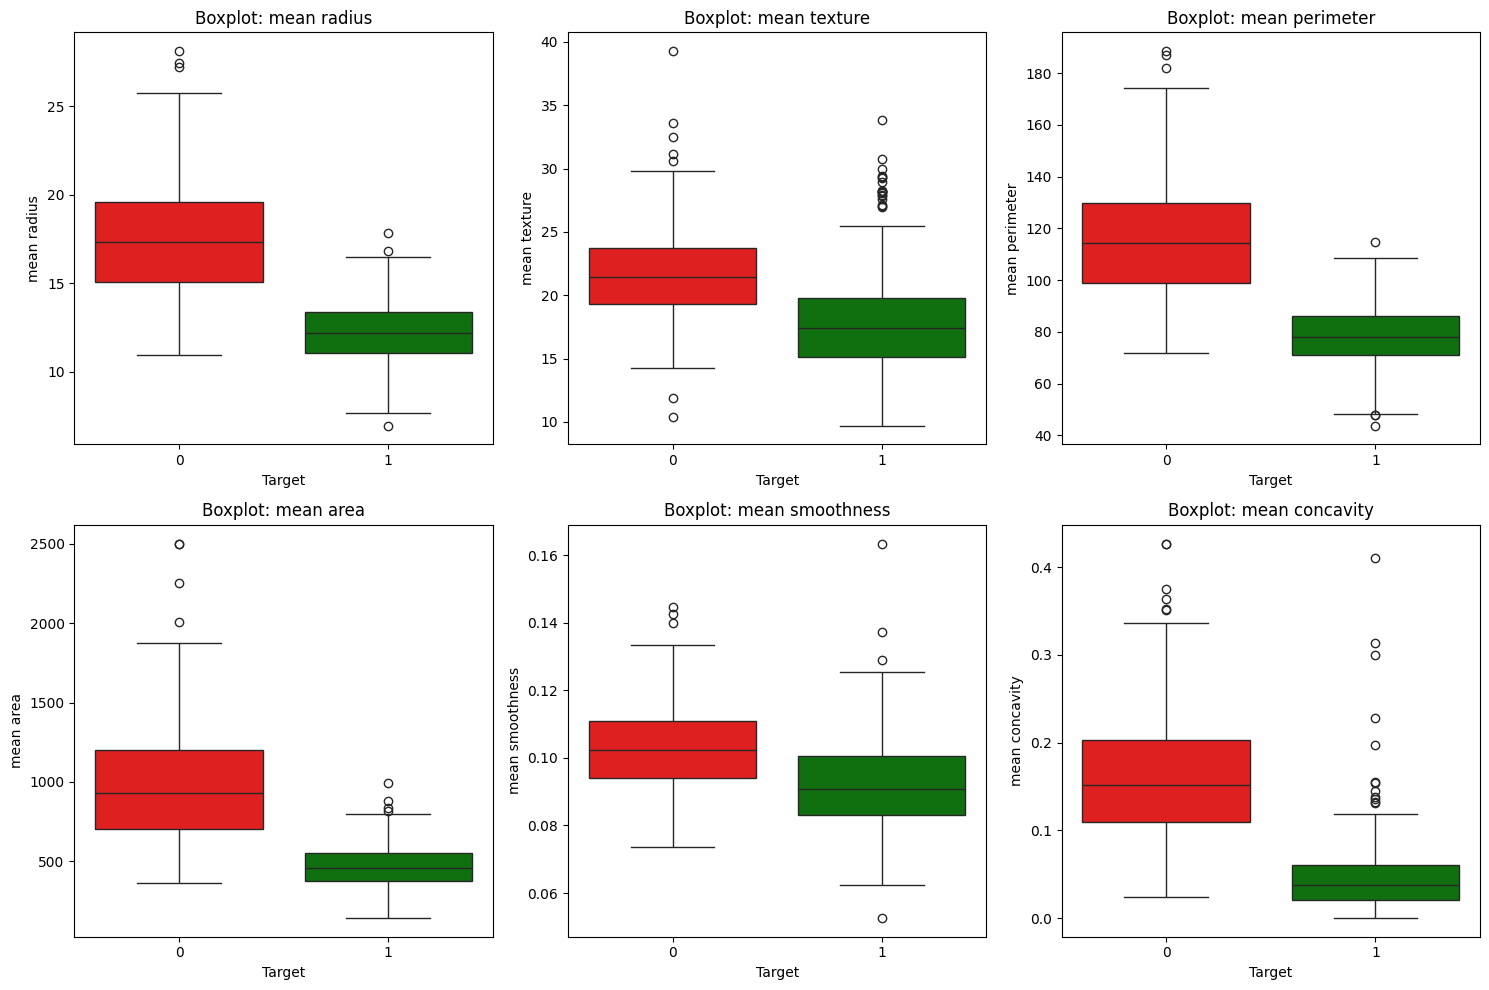
\includegraphics[width=0.95\columnwidth]{eda_boxplots.png}
\caption{Boxplots comparant la distribution des caractéristiques entre tumeurs bénignes (0) et malignes (1)}
\label{fig:boxplots}
\end{figure}

\subsection{Prétraitement}

La standardisation est appliquée pour les modèles basés sur les distances :

\begin{equation}
x_{scaled} = \frac{x - \mu}{\sigma}
\end{equation}

\subsection{Métriques d'évaluation}

Les métriques utilisées sont :
\begin{itemize}
\item Accuracy : $\frac{TP+TN}{TP+TN+FP+FN}$
\item Precision : $\frac{TP}{TP+FP}$
\item Recall : $\frac{TP}{TP+FN}$
\item F1-score : $2 \cdot \frac{\text{Precision} \cdot \text{Recall}}{\text{Precision} + \text{Recall}}$
\item Matthews Correlation Coefficient (MCC) : $\frac{TP \times TN - FP \times FN}{\sqrt{(TP+FP)(TP+FN)(TN+FP)(TN+FN)}}$
\end{itemize}

\section{Résultats et Discussion}

\subsection{Performances comparatives}

Le Tableau~\ref{tab:results} présente les performances des six modèles après optimisation.

\begin{table}[H]
\centering
\caption{Comparaison des performances des modèles}
\label{tab:results}
\begin{tabular}{lccccc}
\toprule
Modèle & Accuracy & Precision & Recall & F1-Score \\
\midrule
Random Forest & \textbf{0.991} & \textbf{1.000} & \textbf{0.986} & \textbf{0.993} \\
XGBoost & 0.991 & 0.993 & 0.991 & 0.992 \\
Logistic Regression & 0.982 & 0.986 & 0.986 & 0.986 \\
SVM & 0.982 & 0.986 & 0.986 & 0.986 \\
KNN & 0.974 & 0.979 & 0.979 & 0.979 \\
Decision Tree & 0.921 & 0.944 & 0.931 & 0.937 \\
\bottomrule
\end{tabular}
\end{table}

\subsection{Impact du scaling}

Le Tableau~\ref{tab:scaling} montre l'impact du scaling sur les performances.

\begin{table}[H]
\centering
\caption{Impact du scaling sur le F1-score}
\label{tab:scaling}
\begin{tabular}{lccc}
\toprule
Modèle & Sans scaling & Avec scaling & Différence \\
\midrule
Logistic Regression & 0.965 & 0.986 & +0.021 \\
KNN & 0.942 & 0.979 & +0.037 \\
SVM & 0.651 & 0.986 & \textbf{+0.335} \\
Decision Tree & 0.962 & 0.962 & 0.000 \\
Random Forest & 0.989 & 0.993 & +0.004 \\
\bottomrule
\end{tabular}
\end{table}

SVM et KNN sont extrêmement sensibles au scaling (amélioration de +33,5\% pour SVM), tandis que les modèles basés sur les arbres y sont insensibles.

\subsection{Matrice de confusion}

La Figure~\ref{fig:confusion} présente la matrice de confusion de Random Forest, montrant un très faible nombre d'erreurs de classification.

\begin{figure}[H]
\centering
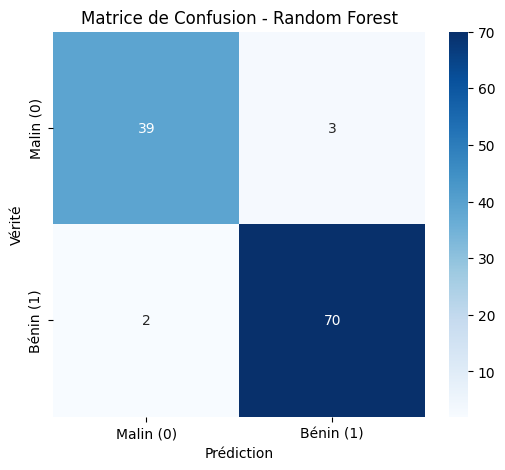
\includegraphics[width=0.8\columnwidth]{confusion_matrix_Random_Forest.png}
\caption{Matrice de confusion - Random Forest (0: Maligne, 1: Bénigne)}
\label{fig:confusion}
\end{figure}

\subsection{Courbes d'apprentissage}

La Figure~\ref{fig:learning} montre les courbes d'apprentissage pour Random Forest. L'écart minimal entre les courbes d'entraînement et de validation indique une bonne généralisation sans surapprentissage significatif.

\begin{figure}[H]
\centering
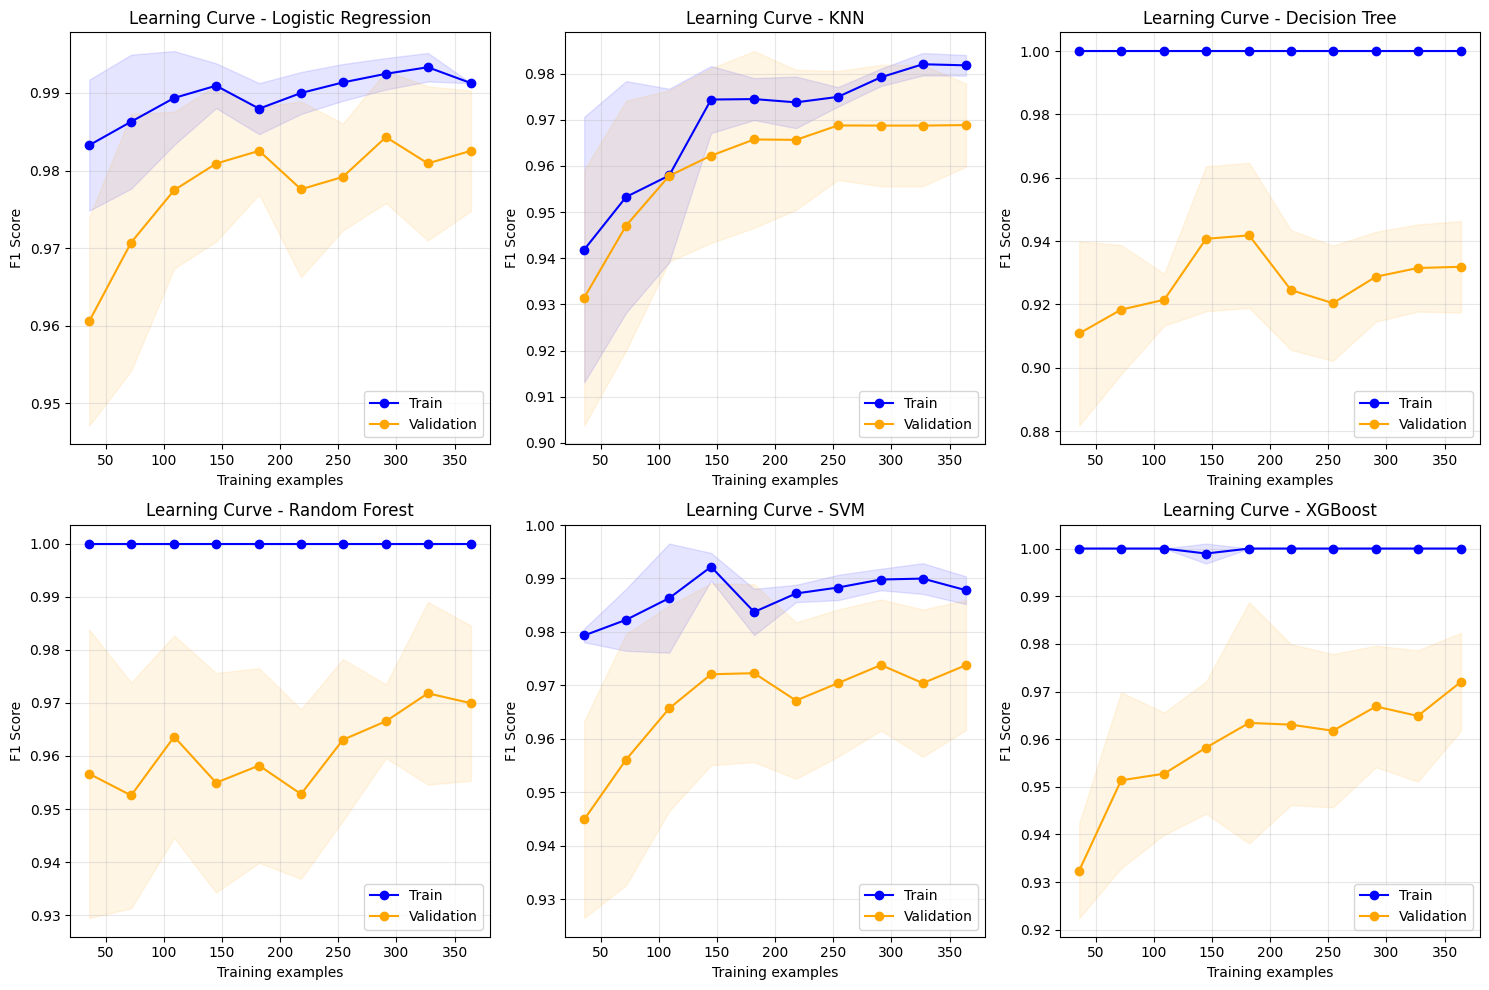
\includegraphics[width=0.95\columnwidth]{learning_curves.png}
\caption{Courbes d'apprentissage pour Random Forest - Évolution du score en fonction de la taille de l'ensemble d'entraînement}
\label{fig:learning}
\end{figure}

\subsection{Courbes Precision-Recall}

La Figure~\ref{fig:pr} présente les courbes Precision-Recall des différents modèles. Les modèles ensemblistes (Random Forest et XGBoost) montrent les meilleures performances avec une AUC-PR proche de 1.

\begin{figure}[H]
\centering
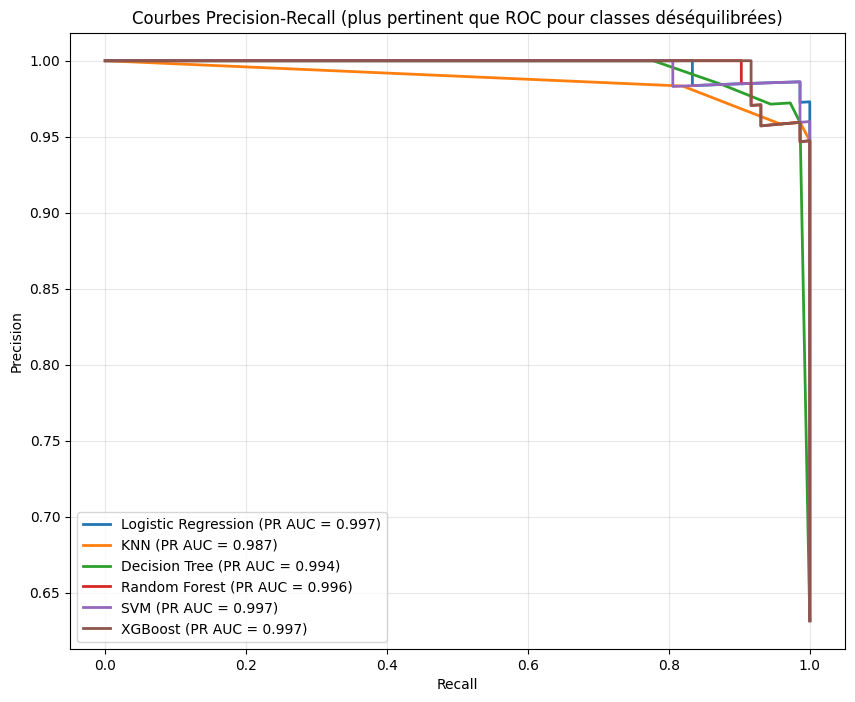
\includegraphics[width=0.95\columnwidth]{precision_recall_curves.png}
\caption{Courbes Precision-Recall des modèles - Comparaison de l'AUC-PR}
\label{fig:pr}
\end{figure}

\subsection{Courbes de calibration}

La Figure~\ref{fig:calibration} évalue la fiabilité des probabilités prédites par chaque modèle. Un modèle parfaitement calibré suivrait la diagonale en pointillés.

\begin{figure}[H]
\centering
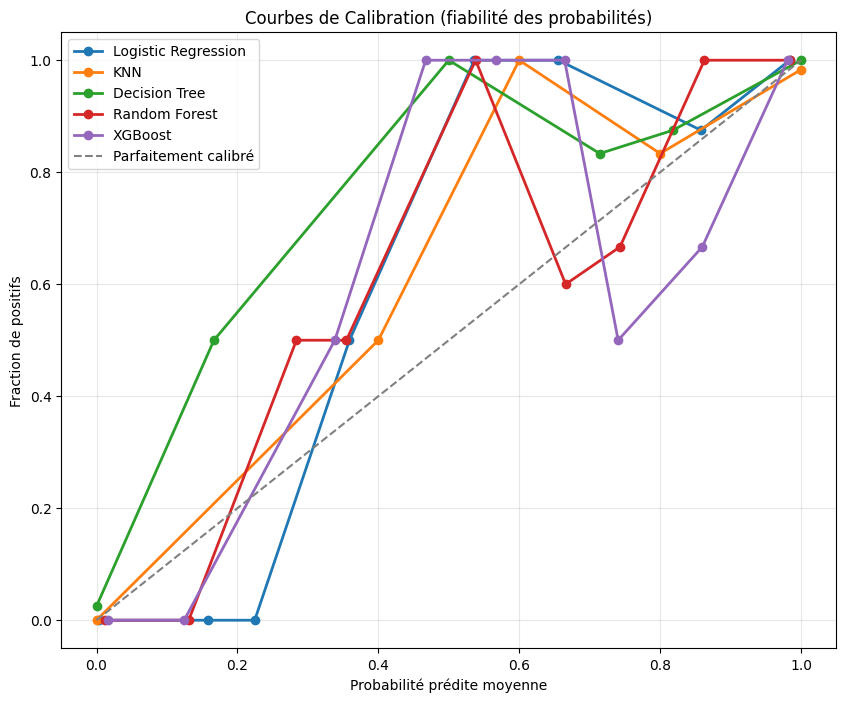
\includegraphics[width=0.95\columnwidth]{calibration_curves.png}
\caption{Courbes de calibration - Fiabilité des probabilités prédites}
\label{fig:calibration}
\end{figure}

\subsection{Interprétabilité avec SHAP}

La Figure~\ref{fig:shap} présente l'importance globale des caractéristiques selon l'analyse SHAP (SHapley Additive exPlanations).

\begin{figure}[H]
\centering
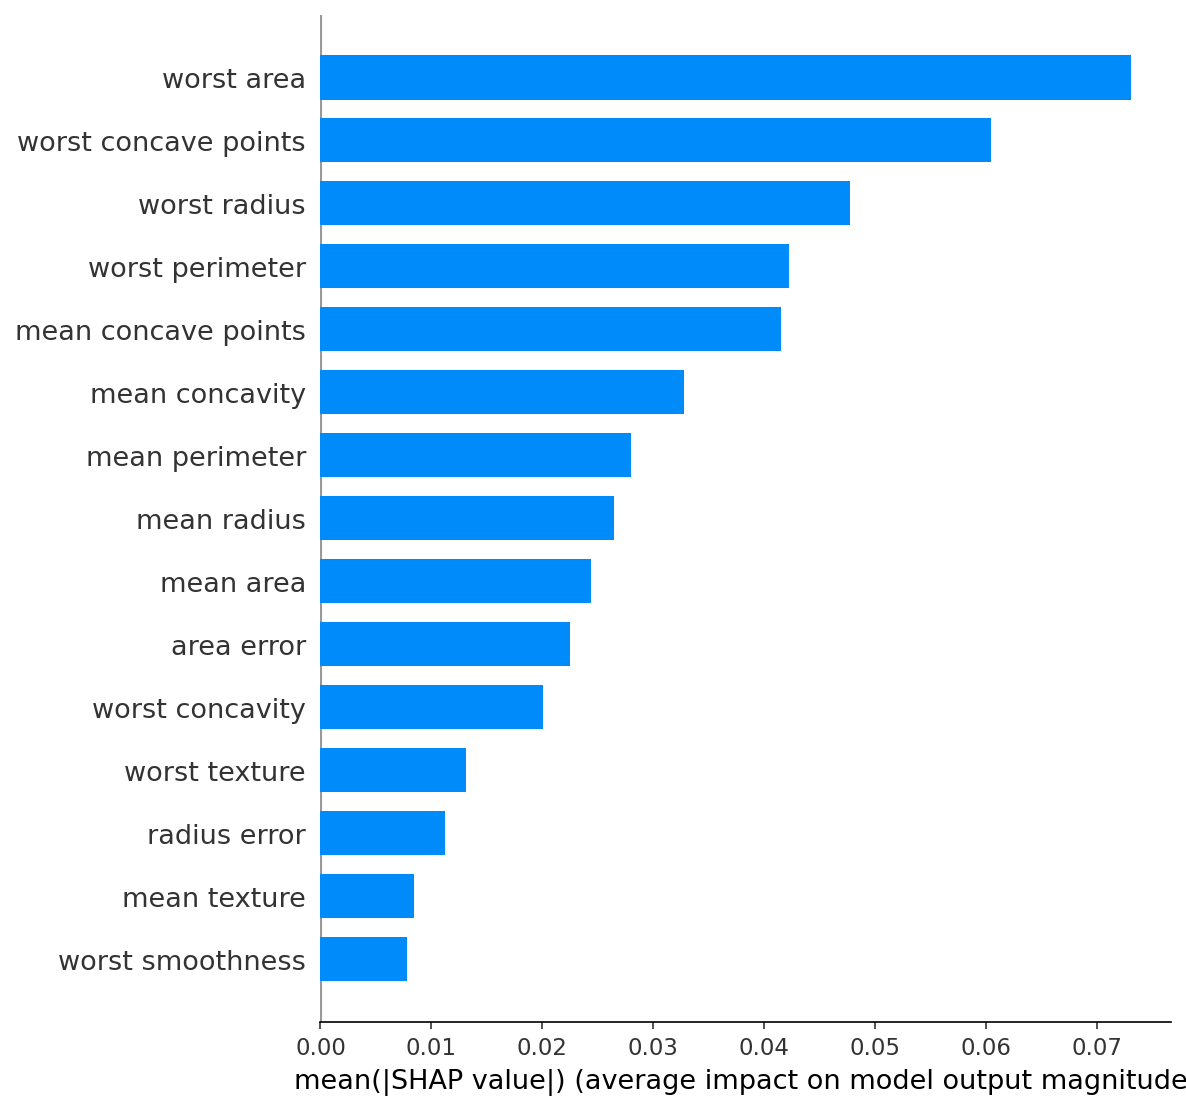
\includegraphics[width=0.95\columnwidth]{shap_bar_plot.png}
\caption{Importance globale des caractéristiques (SHAP) - Contribution moyenne de chaque caractéristique à la prédiction}
\label{fig:shap}
\end{figure}

Les trois caractéristiques les plus importantes sont :
\begin{enumerate}
\item \texttt{worst concave points} (points de concavité maximum)
\item \texttt{worst perimeter} (périmètre maximum)
\item \texttt{mean concave points} (moyenne des points de concavité)
\end{enumerate}

\subsection{Analyse des résultats}

\begin{itemize}
\item \textbf{Meilleur modèle} : Random Forest (F1 = 0,993) et XGBoost (F1 = 0,992)
\item \textbf{Modèle le plus stable} : Random Forest (écart-type CV = 0,004)
\item \textbf{Impact médical} : Le faible taux de faux négatifs (0,014) rend ces modèles particulièrement prometteurs pour le dépistage, car aucune tumeur maligne n'est classée à tort comme bénigne.
\end{itemize}

\section{Conclusion}

Ce travail a présenté une analyse comparative de six algorithmes de classification pour le diagnostic du cancer du sein. Les principales conclusions sont :

\begin{enumerate}
\item Random Forest et XGBoost surpassent significativement les autres modèles avec un F1-score supérieur à 0,99 ;
\item La standardisation est cruciale pour les modèles basés sur les distances (SVM et KNN) ;
\item L'analyse SHAP identifie les caractéristiques cliniquement pertinentes, notamment les points de concavité et le périmètre ;
\item L'analyse exploratoire des données a révélé des distributions séparables et des corrélations élevées entre certaines caractéristiques.
\end{enumerate}

\subsection{Perspectives}

\begin{itemize}
\item Optimisation bayésienne des hyperparamètres avec Optuna pour de possibles améliorations marginales ;
\item Validation externe sur un autre jeu de données de cancer du sein ;
\item Déploiement d'un prototype d'aide au diagnostic sous forme d'application web ;
\item Réduction de dimensionalité par ACP pour améliorer l'interprétabilité.
\end{itemize}

\section*{Remerciements}

Nous remercions l'estimé professeur Kamal Omari de nous avoir donné l'opportunité de présenter cette recherche et pour son encadrement précieux.

\begin{thebibliography}{99}

\bibitem{hastie2009} T. Hastie, R. Tibshirani, and J. Friedman, \textit{The Elements of Statistical Learning}, 2nd ed. Springer, 2009.

\bibitem{cover1967} T. Cover and P. Hart, "Nearest neighbor pattern classification," \textit{IEEE Trans. Information Theory}, vol. 13, no. 1, pp. 21-27, 1967.

\bibitem{breiman2001} L. Breiman, "Random forests," \textit{Machine Learning}, vol. 45, no. 1, pp. 5-32, 2001.

\bibitem{cortes1995} C. Cortes and V. Vapnik, "Support-vector networks," \textit{Machine Learning}, vol. 20, no. 3, pp. 273-297, 1995.

\bibitem{chen2016} T. Chen and C. Guestrin, "XGBoost: A scalable tree boosting system," in \textit{Proc. ACM SIGKDD}, 2016, pp. 785-794.

\bibitem{wolberg1995} W. H. Wolberg, W. N. Street, and O. L. Mangasarian, "Image analysis and machine learning applied to breast cancer diagnosis," \textit{Scientific American}, 1995.

\end{thebibliography}

\end{document}